\chapter{Hasil dan Pembahasan}
\section{Hasil Pengujian}
Setelah melaksanakan pengujian sistem seperti yang telah dibahas pada bab sebelumnya sub bab ini akan memaparkan hasil dari percobaan.
\subsection{Eksistensi Fitur}
%\subsubsection{Pemantauan dan Deteksi}
Pemantauan (aktivitas jantung) dan Deteksi (detak dan aritmia) berhasil dilakukan secara realtime (parameter lainnya, dibahas pada sub bab berikutnya). Berikut beberapa perbandingan mode \textit{monitoring} sistem sejenis lainnya yang berada pada puncak 8 Android Playstore (kata pencarian heart rate) \cite{playstore_heart} ditambah 2 aplikasi medis.

\begin{table}[H]
	\centering
	\begin{tabular}{|l|L{5cm}|c|L{0.5cm}|L{0.5cm}|L{0.5cm}|L{0.5cm}|L{0.5cm}|L{0.5cm}|L{0.5cm}|L{0.5cm}|}
		\hline
		\rowcolor{gray}
		\textbf{No} & \textbf{Produk} & \textbf{Sen} & \multicolumn{8}{c}{\textbf{Fitur}} \\
		\rowcolor{gray}
		 & & \textbf{sor} & A & B & C & D & E & F & G & H \\
		\hline
		1 & Tugas Akhir & PPG & Y & Y & Y & Y & Y & Y & Y & N \\
		2 & Instant Heart Rate : Heart Rate \& Pulse Monitor & PPG & Y & N & Y & Y & N & Y & N & Y \\
		3 & iCare Health Monitor (BP \& HR) & PPG & Y & N & Y & N & N & Y & N & Y \\
		4 & Heart Rate Monitor(REPS) & PPG & Y & N & Y & Y & N & Y & N & Y \\
		5 & Runtastic Heart Rate Monitor \& Pulse Checker & PPG & Y & N & Y & N & N & Y & N & N \\
		6 & Cardiograph - Heart Rate Meter & PPG & Y & N & Y & Y & N & Y & N & Y \\
		7 & ASUS Heart Rate & PPG & N & N & N & N & N & Y & N & N \\
		8 & Samsung Health & PPG & Y & Y & N & N & N & Y & N & Y \\
		9 & Heart Rate Monitor(Meet Your Need Production) & PPG & N & N & N & N & N & Y & N & N \\
		10 & \textbf{MobECG} & \textbf{ECG} & N & Y & Y & Y & N & Y & N & N \\		
		11 & \textbf{CMS50Dplus} & \textbf{ECG} & N & Y & Y & Y & N & Y & N & N \\
		\hline
	\end{tabular}
\end{table}

Ket: \\
A = Identitas User \\
B = Real Time Monitoring \\
C = Melihat Gelombang Jantung \\
D = Merekam Gelombang Jantung \\
E = Multiuser Monitoring \\
F = Deteksi BPM \\
G = Aritmia Alert \\
H = Share Result \\

\subsection{Delay}
Pengujian dilakukan oleh pengguna yang bergerak secara bebas dalam wilayah cakupan router (\textit{receptor}, \textit{router} dan \textit{server} masih dalam satu wilayah) sehingga tidak ada proses routing antara router. Setelah melakukan pengujian sebanyak 3 kali pada waktu berbeda (pagi, siang, malam) didapatkan rata-rata delay percobaan-1 1.60624 ms, percobaan-2 1.36287 ms dan percobaan-3 1.45066 ms. Hasil pengukuran delay tertera pada gambar \ref{fig:delay}. Rata-rata ketiga percobaan ialah 1.47326 ms per sampel.

\begin{figure}[H]
	\centering
	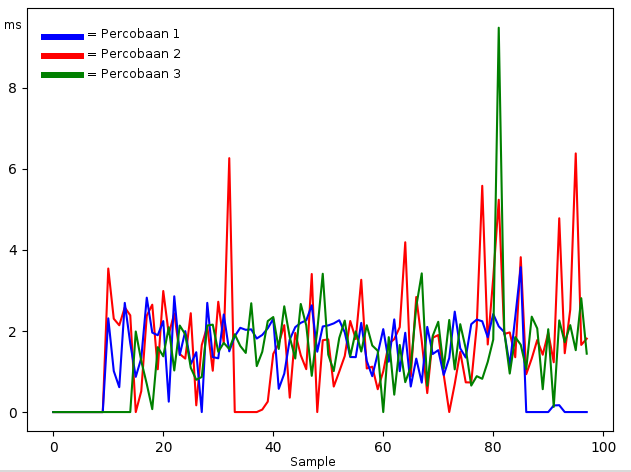
\includegraphics[scale=0.5]{images/delay1.png}
	\caption{Hasil Pengukuran Delay 100 sample}
	\label{fig:delay}
\end{figure}

\subsection{Execution Time}
Hasil pengukuran execution time tertera pada grafik ...

\subsection{FPS}
Setelah melakukan pengujian, ditemukan FPS terbaik untuk dapat berjalan dengan lancar pada kedua jenis \textit{viewer} yaitu 20 FPS. Hasil lengkap percobaan FPS dapat dilihat pada tabel ...

\begin{table}[H]
	\centering
	\begin{tabular}{|l|l|l|l|}
	
	\end{tabular}
\end{table}

\subsection{Akurasi}
Setelah melakukan pengujian didapatkan hasil akurasi xx\% untuk detaksi detak dan xx\% untuk deteksi aritmia.
\subsubsection{Akurasi Detak}
Dilakukan percobaan untuk menemukan konfigurasi konstanta deteksi $\alpha$, $\beta$ dan $d$ (durasi window).
\subsubsection{Akurasi Aritmia}

\section{Pembahasan}
Dengan terdapatnya mode \textit{monitoring} maka parameter 1 (Eksistensi Fitur) dinyatakan terpenuhi.


\textit{Delay} dan \textit{Execution time} ini terhitung kecil sehingga tidak menyebabkan fenomena \textit{bottleneck} pada sisi server.